\subsection{Internet}

In both cases, a \gls{pppoe} connection must be established with the proper credentials. The \gls{vlan} \gls{id} must be set to 600 and \gls{ip}v6 can be enabled with \gls{slaac}.

When setting up the devices for the first time, or after a factory reset, a Quick Setup page, shown in Figure \ref{figure:crgs_quicksetup}, is presented when the \gls{http} Management Interface is accessed.

\begin{figure}[h]
    \centering
    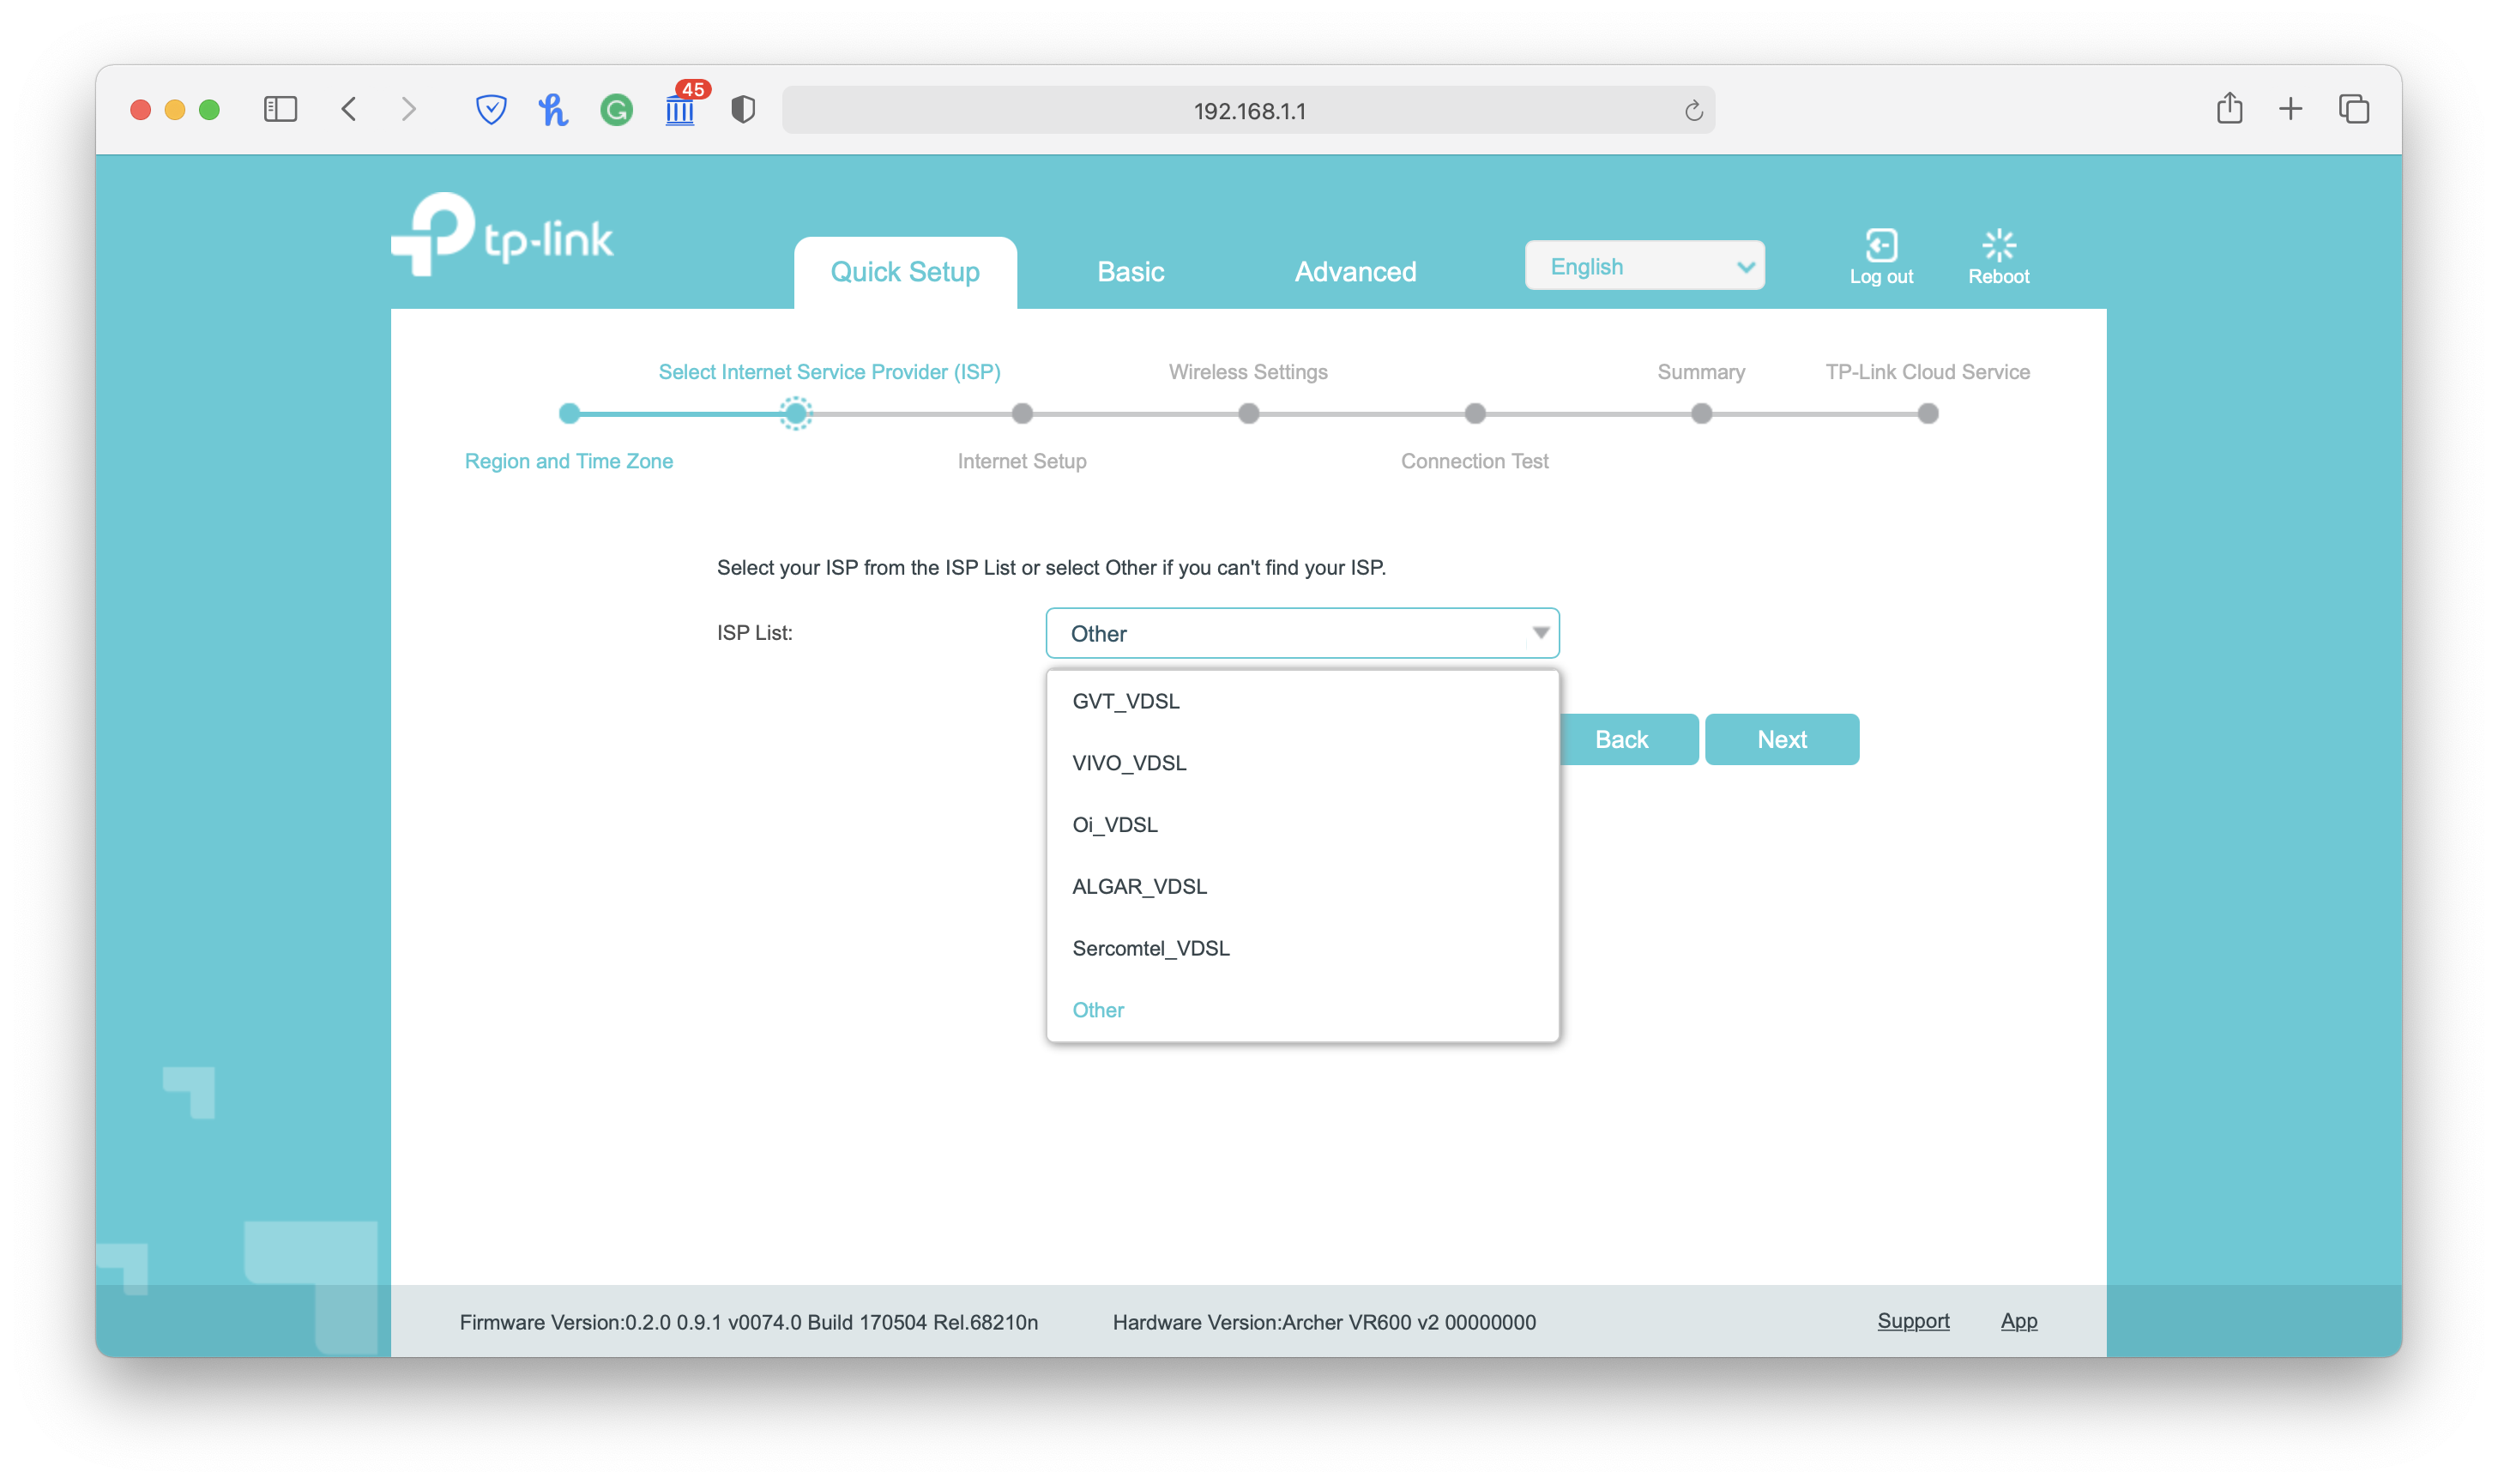
\includegraphics[width=\linewidth]{contents/substituting-the-isp-cpe/internet/quick-setup.png}
    \caption{Quick Setup of the \gls{crg}s}
    \label{figure:crgs_quicksetup}
\end{figure}

In the case of \gls{crg}-0, the setup page contains a list of \glspl{isp} that the device can be automatically configured to work with. Although the \gls{isp} being analyzed shows on the list, the autoconfiguration doesn’t work as expected and the residential gateway is not able to connect to the Internet. But also on the list, is an \gls{isp} that was acquired and incorporated by the researched provider and selecting it for autoconfiguration makes the equipment connect to the network.

\gls{crg}-1 doesn’t have a predefined list of \glspl{isp} like \gls{crg}-0, but it can be easily configured with the required information. This process can also be performed on \gls{crg}-0 with almost no difference.

\begin{figure}[h]
    \centering
    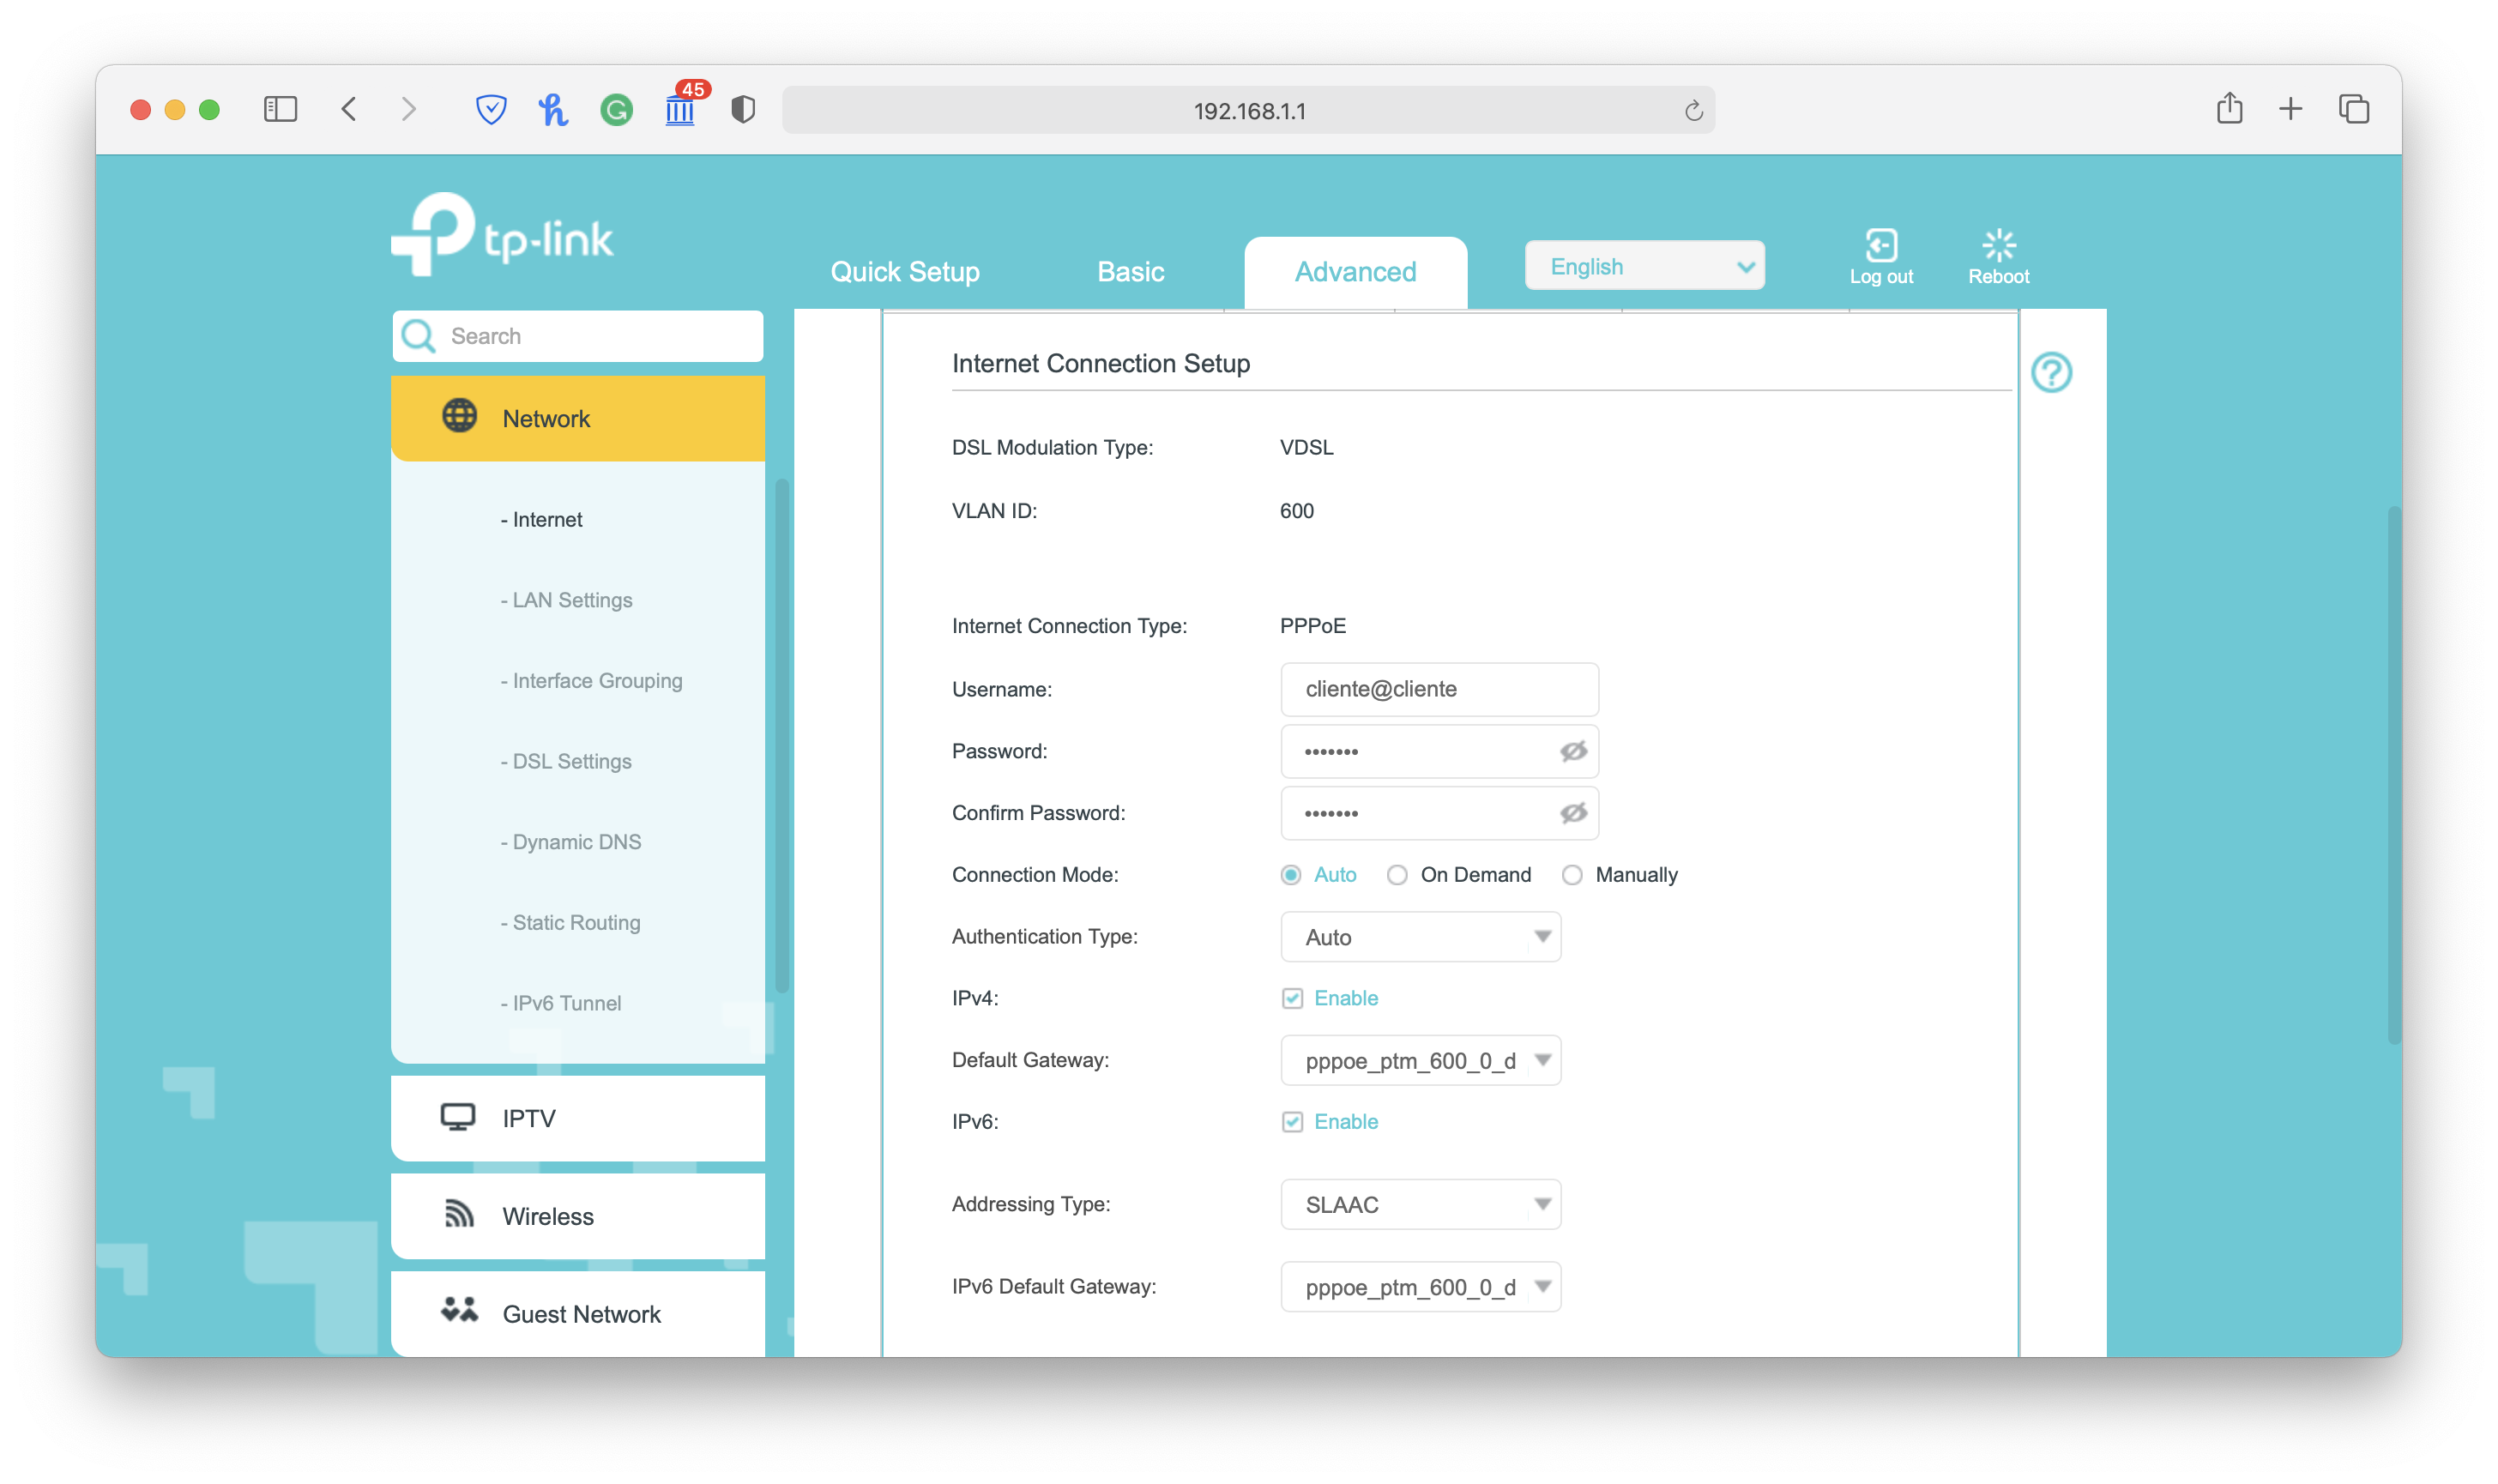
\includegraphics[width=\linewidth]{contents/substituting-the-isp-cpe/internet/advanced-network-internet-vlan600.png}
    \caption{\gls{vlan} 600 Settings of the \gls{crg}s}
    \label{figure:crgs_vlan600}
\end{figure}

In the advanced section of the device’s web interface, there is a page that allows Internet Connections to be manually configured. By clicking on the add button, the \gls{vlan} \gls{id} must be set to 600 and the Connection Type to \gls{pppoe}, as shown in Figure \ref{figure:crgs_vlan600}. The credentials for the \gls{pppoe} connection are the same found hard-coded on all \glspl{cpe} inspected.

In fiber-based devices, you are also required to enter the \gls{gpon} \gls{s/n}, that could be found on the about page on the \gls{http} Management Interface of all fiber-based \glspl{cpe} analyzed. While in copper-based devices, the \gls{dsl} Modulation Type must be set to \gls{vdsl}.

Optionally, \gls{ip}v6 can be enabled with \gls{slaac}, but it depends on regional availability to work. The experiment showed that \gls{ip}v6 works on devices located in the Metropolitan Area of the state, but it does not on the Agreste Region.

\FloatBarrier
